\chapter{Metode za razvoj grafično intenzivnih medplatformnih aplikacij}

Ogledali si bomo različne metode in orodja, ki so na voljo za razvoj grafično intenzivnih medplatformnih aplikacij. Kot prvi primer pisanja medplatformnih aplikacij bomo obravnavali spletne aplikacije, saj so spletni brskalniki prisotni na večini platform. Ogledali si bomo tudi kako spletne aplikacije izvajati kot namizne aplikacije brez brskalnika. Preučili bomo, kako s programskim jezikom Java in orodjem Xamarin razvijamo medplatformne aplikacije. Zanimalo nas bo tudi orodje Unity, ki omogoča preprost izvoz aplikacij za različne platforme. Dotaknili se bomo tudi programskega jezika Haxe, ki je bil ustvarjen z razlogom, da bi olajšal razvoj medplatformnih aplikacij. Na koncu poglavja si bomo ogledali še razvoj grafično intenzivnih aplikacij v programskih jezikih C++, C\# in ActionScript.

\section{Spletne aplikacije}
\label{sec:web}
Programski jezik JavaScript je nastal okoli leta 1995, ko je bil tudi vključen v spletni brskalnik Netscape. Jezik JavaScript je omogočil izvedbo kode na uporabnikovi strani (angl. client-side) in spletne strani so postale interaktivne.

V zgodnjih dneh spleta se programiranje na uporabnikovi strani ni veliko uporabljalo. Javscript interpreterji so bili počasni, zaradi neenotnih standardov med brskalniki pa je bilo pisanje aplikacije, ki bi delala enako na vseh, zelo težavno. Šele kasneje, ko so brskalniki malo napredovali, je postalo pisanje aplikacij na strani uporabnika dejanska opcija.

S pojavom spletnega brskalnika Google Chrome se je začela nova doba brskalnikov in bogatih aplikacij na strani uporabnika. Google Chrome je začel pravo tekmo za hitrost. Ker so spletne aplikacije postajale vedno bolj zahtevne, je bilo prvenstvenega pomena, da brskalniki postanejo hitri in odzivni.

Brskalniki so začeli med seboj tekmovati, kdo lahko hitrejše izvaja JavaScript izvorno kodo. Rezultat te tekme pa je bil, da so v roku parih let vsi novejši brskalniki sposobni hitro izvajati tudi bolj zahtevne JavaScript aplikacije. 

S pojavom pametnih telefonov in tablic so spletne tehnologije postale dostopne tudi na mobilnih platformah. Zaradi strojnih omejitev in predvsem življenjske dobe baterij, so bili hitri in učinkoviti JavaScript pogoni na mobilnih platformah celo bolj pomembni kot na namiznih računalnikih.

Kot rezultat vseh prizadevanj za izboljšanje učinkovitosti in hitrosti izvajanja izvorne kode spletnih strani, lahko danes tako na namiznih računalnikih in mobilnih napravah izvajamo zahtevne aplikacije, ki se izvajajo znotraj spletnega brskalnika.

Programski jezik JavaScript je pravzaprav ena izmed redkih skupnih točk pametnih telefonov, tablic in namiznih računalnikov. Za razvoj domorodnih aplikacij za specifične naprave je potrebno uporabljati programski jezik, ki je določen s strani proizvajalca. Prav vse mobilne naprave pa imajo naložen brskalnik, v katerem lahko poganjamo spletne aplikacije napisane v JavaScriptu.

Prav vse mobilne platforme imajo tudi takšno ali drugačno implementacijo tako imenovanega elementa za spletni pogled (angl. webview). Ta element nam omogoča prikaz določene spletne strani znotraj domorodne aplikacije. Na ta način lahko spletno aplikacijo zapakiramo v ovitek, ki se potem iz vidika končnega uporabnika obnaša slično domorodnim aplikacijam. Zanimiva izjema je Mozillin mobilni operacijski sistem Firefox OS, ki spletne aplikacije smatra kot domorodne in zato ne potrebuje posebnega ovitka.

\subsection{2D platno}
\label{sec:2dcanvas}
Sodobni brskalniki nam za izris svojih oblik na zaslon poleg HTMLja in CSSa ponujajo tudi uporabo platna (angl. canvas) \cite{canvas}. 

Element platno se je pojavi kot Appleov eksperiment znotraj Mac OSX Webkit komponente leta 2004. Uporabljen je bil v spletnem brskalniku Safari in za vtičnike v Dashboard aplikaciji. Leto kasneje so podporo platnu dodali tudi Gecko brskalniki, leta 2006 pa tudi spletni brskalnik Opera. Istega leta je organizacija Web Hypertext Application Technology Working Group (WHATWG) element standardizirala. Internet Explorer je dodal domorodno podporo za platno v verziji 8.

Platno je danes dobro podprto v vseh modernih spletnih brskalnikih, tudi na mobilnih napravah. Na določenih platformah in brskalnikih lahko uporablja tudi strojno pospeševanje, vendar se ta funkcija zaenkrat smatra še kot eksperimentalna in praviloma ni dostopna povsod. Zaradi slabe strojne podpore obstajajo omejitve kompleksnosti, ki jih s platnom lahko dosežemo.

% http://www.html5rocks.com/en/tutorials/canvas/performance/

Platno je namenjeno izrisovanju dvodimenzionalnih oblik na zaslon. Programerju nudi preprost vmesnik API za risanje raznih oblik (\texttt{fillRectn}, \texttt{fillCircle}), risanje besedila (\texttt{fillText}), risanje poti (\texttt{moveTo}, \texttt{lineTo}), risanje slik (\texttt{drawImage}) in tudi risanje gradientov (\texttt{drawGradient}). Nudi tudi dostop do operacij nad posameznimi oblikami, kot so na primer premakni (\texttt{translate}), zavrti (\texttt{rotate}). 

Programer lahko aplikacijo s platnom razvija in testira na namiznem računalniku. Vmesne rezultate dela lahko preverja v svojem spletnem brskalniku in šele nato, ko se prepriča v pravilno delovanje, prenese aplikacijo na mobilno napravo. Ta način dela zelo pohitri razvoj, saj prenos aplikacije na mobilno napravo traja več časa. Pri razvijanju aplikacije na namiznem računalniku mora biti programer še posebej pozoren na strojne omejitve mobilnih naprav. 

Prednost uporabe dvodimenzionalnega platna je, v dobri medplatformni podpori tako na namiznih računalnikih kot tudi na mobilnih napravah. Cena dobre podprtosti pa so omejene zmožnosti. Izrisovanje zahtevnejših slik lahko postane počasno, izrisovanje v treh dimenzijah pa zaradi slabe podpore strojnemu pospeševanju skorajda nemogoče. 

Kljub pomanjkljivostim lahko s pomočjo platna na preprost način napišemo grafično intenzivno aplikacijo, ki bo delala na več platformah. 

\subsubsection{Strojno pospeševanje}

Dvodimenzionalno platno na določenih konfiguracijah omogoča tudi strojno pospeševanje. Z omogočenim strojnim pospeševanjem centralna procesna enota prenese nekaj svojega dela na grafično procesno enoto. Na ta način se lahko hitrost izrisovanja močno poveča.

Strojno pospešeno platno zaenkrat še ni na voljo povsod in zato na prednosti, ki jih prenaša, še ne gre računati. Brskalnik Google Chrome je na primer dodal podporo v verziji 18 (Marec 2012), vendar strojno pospeševanje še vedno ni omogočeno na platformah Linux in Android.

\subsection{3D platno WebGL}
\label{sec:WebGL}

WebGL \cite{webgl} je medplatformni programski vmesnik, uporabljen za delo s tridimenzionalno grafiko znotraj spletnega brskalnika. Je kontekst platna, ki ima direkten dostop do grafične kartice preko GLSL jezika za pisanje programov, ki se izvajajo direktno na grafični kartici. Ti programi se imenujejo senčilniki (angl. shaders). 

WebGL temelji na OpenGL ES 2.0 standardu in je na voljo na namiznih računalnikih in na nekaterih mobilnih napravah. Podpora OpenGL ES 2.0 na mobilni napravi še ne pomeni, da naprava podpira WebGL. Tak primer je iOS, ki WebGL standarda zaenkrat še ne podpira.

WebGL je nastal iz eksperimentov Vladimira Vukićevića, zaposlenega pri Mozilli. Leta 2006 je začel delati na pospešenem "3D platnu za splet". Do konca leta 2007 sta tako Mozilla kot Opera imeli delujočo implementacijo WebGL vmesnika API. Leta 2009 je neprofitna organizacija Khronos ustanovila skupino za delo na WebGLu (WebGL Working Group). Člani skupine so bili tudi Apple, Google, Mozilla, Opera in drugi. Prva verzija specifikacije je bila izdana marca 2011.

Mozilla je dodala podporo WebGLu v Firefoxu 4.0, Google v Chromu od verzije 9 naprej, Apple je dodal podporo v Safari 6.0, v Operi pa se je podpora pojavila v verziji 11, vendar je bila privzeto izklopljena. Internet Explorer je dodal podporo WebGLu šele v verziji 11, ki je v času pisanja na voljo samo kot predogled v okviru Windows 8.1 verzije za razvijalce.

Na mobilnih brskalnikih je stanje še slabše. Večina mobilnih brskalnikov še nima vgrajene podpore (Safari na iOS) ali pa je le ta še v fazi preizkušanja (Chrome na Androidu). WebGL je najbolje podprt v mobilni različici brskalnika Firefox.

WebGL, za razliko od dvodimenzionalnega platna, brez strojne podpore sploh ne deluje. 

WebGL kompatibilnost ima svoje probleme tudi na namiznih računalnikih, saj na določenih kombinacijah operacijskih sistemov, grafičnih kartic in brskalnikov še vseeno ne deluje. Problem je, da je še vedno veliko gonilnikov za grafične kartice na črni listi, ki ima delovanje privzeto izklopljeno. Na črni listi so gonilniki, ki po mnenju avtorjev brskalnikov še niso dovolj stabilni oziroma imajo pri prikazovanju WebGL vsebin težave. Omejitve sicer lahko zaobidemo s postavitvijo posebne zastavice ob zagonu brskalnika, vendar s tem lahko tvegamo anomalije pri prikazovanju ali celo nestabilnost brskalnika.

Razvijalci brskalnikov kot glavni razlog za slabo podprtost WebGLa navajajo probleme z varnostjo. Narediti peskovnik (angl. sandbox) za spletno stran ni trivialno, še posebej če le ta za svoje delovanje potrebuje direkten dostop do grafične kartice.

\subsubsection{Razvoj WebGL aplikacije}

Razvoj aplikacij z uporabo WebGLa je bolj zahtevno za programerja, kot razvoj aplikacij z 2D platnom. WebGL programski vmesnik namreč ne omogoča preprostih funkcij za risanje na zaslon in tudi za izris najbolj osnovnih oblik je potrebno kar nekaj dela. Nastaviti je potrebno pravilen kontekst in napisati, prevesti ter povezati dva programa senčilnika. 

Senčilniki so programi, ki se izvajajo na grafični procesni enoti. WebGL definira dve vrsti senčilnih programov - ogliščni (angl. vertex) in fragmentni (angl. fragment). Prvi skrbi za pozicijo vsakega oglišča, ki ga izrišemo na na zaslonu, drugi pa za barvo vsakega fragmenta. Pisanje senčilnikov poteka v programskem jeziku GLSL, ki je podzvrst programskega jezika C. Nabor ukazov je v primerjavi s programskim jezikom ANSI-C sicer omejen, vendar so dodani posebni ukazi za lažje delo z vektorji in matrikami.

Podobno kot za dvodimenzionalno platno velja tudi za WebGL, aplikacijo razvijamo na namiznem računalniku in po potrebi preizkušamo kompatibilnost na mobilnih napravah.

\subsubsection{Medplatformnost}

V času pisanja WebGL še ni dobra izbira za medplatformni razvoj aplikacij. Vendar vse smernice kažejo, da se bo podpora v prihodnosti precej izboljšala. Dober indikator je tudi vključitev podpore v Internet Explorer 11, kljub dejstvu, da sta bila skupina Khronos in Microsoft v nenehni tekmovalnosti.

Za razliko od zaprtih sistemov, kot je na primer Flash, ki mu podprtost pada\footnote{Adobe Flash na iOSu ni bil podprt nikoli, na Androidu pa v zadnjih verzijah tudi uradno ni več podprt.}, je WebGL trenutno na dobri poti, da postane primerno orodje za razvoj grafično intenzivnih medplatformnih aplikacij.

\subsection{Zvok}

Aplikacije napisane v 2D platnu in aplikacije pisane v WebGLu dostopajo do zvoka na enak način - to zato, ker je izrisovanje povsem ločeno od ostalih komponent.

HTML5 definira dokaj preprost vmesnik API za predvajanje zvočnih datotek znotraj brskalnika. Programer ima na voljo ukaze za predvajanje zvoka, premikanje po zvočni datoteki in nastavljanja glasnosti zvočne datoteke, ne pa tudi kakšnih bolj naprednih ukazov kot spreminjanje frekvence ali tonalitete.

Za bolj napredne funkcije je potrebno poseči po drugih metodah. Ena izmed najbolj uporabnih je uporaba Flash predvajalnika. S tem pridobimo dodatne funkcije za delo z zvokom, vendar se zaradi vse slabše podpore Flash predvajalnikov na mobilnih napravah tudi lahko precej omejimo. 

Uporabimo lahko tudi knjižnico, ki nam za predvajanje zvoka ponudi svoj lasten vmesnik API in potem zvoke predvaja na najboljši način glede na dano platformo, na kateri se aplikacija izvaja. Taka knjižnica je tudi SoundJS \cite{soundjs}, ki glede na zmogljivosti platforme zvok predvaja z vmesnikom WebAudio ali s pomočjo \texttt{<audio>} HTML elementa. Na voljo je tudi pritiklina za predvajanje zvoka s Flash predvajalnikom.
 
\subsection{Zaznavanje vhoda}

Grafično intenzivne aplikacije se morajo odzivati tudi na vhod uporabnika. Za vhod je na namiznih računalnikih značilna kombinacija miška in tipkovnica, na mobilnih napravah pa imamo navadno na voljo samo na dotik občutljiv zaslon. V JavaScriptu je napisanih kar nekaj knjižnic, ki nam pomagajo premostiti razlike med različnimi načini vnosa.

\subsection{Primernost programskega jezika JavaScript}

Za razvoj grafično zahtevnih aplikacij je hitrost izvajanja programa bistvenega pomena. Za ta namen se praviloma uporablja statično tipizirane jezike in ročno sproščanje pomnilnika. V industriji je najbolj pogosto uporabljen programski jezik C++.

Kljub vsem izboljšavam in pohitritvam, ki jih danes najdemo v modernih spletnih brskalnikih, je hitrost izvajanja programa napisanega v programskem jeziku JavaScript, še vedno bistveno počasnejša. Razni testi kažejo, da je ekvivalenten program napisan v programskem jeziku C++ lahko tudi do 5 krat hitrejši \cite{jsperformance}.

S pomočjo tehnologij, kot je ASM.js (razdelek \ref{sec:asm}) je možno JavaScript program pohitriti, vendar je kljub temu povprečna hitrost izvajanja še vedno dvakrat počasnejša od ekvivalentnega C++ programa.

Gledano izključno iz vidika hitrosti izvajanja, bo JavaScript najbrž vedno manj primeren od klasičnih jezikov.

\section{Spletne aplikacije z V8-GL}

V8-GL je knjižnica, ki omogoča razvoj grafičnih aplikacij za namizne računalnike v jeziku JavaScript. Knjižnica programerju nudi JavaScript vmesnik do OpenGL vmesnika API. Njen glavni cilj je narediti bogato orodje, ki bo olajšalo delo z 2D in 3D grafiko \cite{v8gl}.

Knjižnica je trenutno še globoko v razvoju in zaenkrat stabilna verzija še ni bila izdana. OpenGL ES 2.0 povezave so že delujoče in na voljo za uporabo. To pomeni, da lahko delujočo WebGL prenesemo na V8-GL in se znebimo odvisnosti od brskalnika. Še vedno veljajo enake omejitve s hitrostjo izvajanja, kot veljajo znotraj brskalnika, vendar nam ni več potrebno skrbeti za delovanje v različnih brskalnikih.

Delo poteka tudi na prevedbi knjižnice za sistema iOS in Android. To bi omogočilo bolj konsistentno medplatformno delovanje aplikacije na več platformah.

\subsection{LycheeJS}

Perspektivna uporaba V8-GL knjižnice je trenutno projekt LycheeJS. LycheeJS je pogon v JavaScriptu, ki teoretično lahko teče na vseh okoljih kjer je na voljo JavaScript  \cite{lycheejs}. LeechJS podpira vse moderne brskalnike na namizju (Firefox, Chrome, Opera, Safari in Internet Explorer) in tudi v mobilnih brskalnikih (WebKit, Firefox, Chrome na Androidu in Mobile Safari). 

Ker se LycheeJS za 3D zmogljivosti zanaša na V8-GL, veljajo enake omejitve pri uporabi OpenGL ES 2.0 APIja kot pri V8-GL. LycheeJS je zgolj ogrodje zgrajeno nad V8-GL-om, ki programerju omogoči abstrakcijo in lažje pakiranje aplikacije. Med prednostmi, ki jih LycheeJS prinaša so ogrodje za delo z 2D grafiko, enoten vmesnik za detekcijo vhoda uporabnikov in enoten vmesnik za predvajanje zvočnih datotek. Orodja za pakiranje aplikacij, ki so vključene v projekt LycheeJS, omogočajo pakiranje aplikacije za različne platforma z enim samim ukazom. Trenutno podprte platforme so spletne aplikacije, vtičniki za brskalnik Google Chrome, namizna aplikacija ter Android aplikacija. Seznam aplikacij pa se bo v prihodnosti še povečal.

\section{Xamarin}
\label{sec:xamarin}

Xamarin nam omogoča, da medplatformno aplikacijo napišemo v programskem jeziku C\#. Znotraj programskega jezika C\# imamo na voljo posebni programski vmesniki, s katerimi lahko dostopamo do knjižnic na domorodnih platformah. Na voljo imamo tudi funkcije iz .NET ogrodja, saj C\# prevajalnik našemu programu doda .NET rutino (Mono). Prevajalnik proizvede izvedljiv program za ARM procesorje, ki je lahko zapakiran kot iOS ali Android aplikacija. Na ta način lahko delimo del izvorne kode med Android in iOS aplikacijami. Določen del kode pa mora vseeno biti ločen, saj Xamarin ne ponuja skupne abstrakcije nad iOS in Android sistemom. 

Xamarin kodo prevede v domorodno izvedljivo binarno datoteko za posamezno platformo. Izvajanje binarne datoteke je hitro in ni vidnih vplivov na hitrost izvajanja \cite{xamarin}. Izvorna koda .NET rutine nam sicer prinese dodatnih 2.5MB podpisa, vendar to danes ne predstavlja večjega problema.

Xamarin temelji na odprtokodni verziji .NET ogrodja - Mono, ki deluje na platformah Linux, Unix, FreeBSD in MacOSX. Za iOS so razvili lasten prevajalnik, ki izvorno kodo v ARM zbirni jezik prevede pred časom (angl. ahead of time). Na operacijskem sistemu Android Xamarinov prevajalnik prevede kodo v vmesni jezik (IL), ki se nato prevede ob pravem času (angl. just in time), ko se aplikacija zažene. V obeh primerih Xamarin poskrbi za dodeljevanje spomina, sproščanje pomnilnika in osnovne komponente platforme. %underlying platform interop, etc. 

Pisanje grafičnih aplikacij z Xamarinom je sicer mogoče, vendar nam Xamarin pri razvoju le malo pomaga. Kot bomo videli v nadaljevanju je Xamarin bolj uporaben kot vmesna plast. Tako ogrodje LibGDX (razdelek \ref{sec:libgdx}) kot PlayN (razdelek \ref{sec:playn}) uporabljata Xamarin za grajenje aplikacije za iOS platformo.

Uporaba Xamarina prevajalnika je sicer možna brez plačila, vendar je velikost aplikacije omejena. Za neomejeno velikost aplikacije je potrebno kupiti eno od plačljivih licenc. Najcenejša licenca, ki omogoča prevajanje večjih aplikacij stane \$299 na posamezno platformo.

\section{LibGDX}
\label{sec:libgdx}
LibGDX \cite{libgdx} je v Javi napisano ogrodje za medplatformni razvoj grafičnih aplikacij. Knjižnica abstrahira razlike med namiznimi računalniki, Androidom, iOSom in spletnimi aplikacijami ter gradi na odprtih standardih, kot sta OpenGL ES in WebGL.

LibGDX omogoča hitro izgradnjo prototipov, saj je razvoj mobilnih aplikacij možen na namizju. V pravilnost delovanja aplikacije se lahko prepričamo iz namiznega računalnika in šele nato zgradimo paket za želeno mobilno napravo. 

Prednost tega pristopa je krajši čas razvijanja aplikacije. Vsake spremembe nam ni potrebno preveriti tudi na mobilni napravi. Grajenje iOS ali Android paketa namreč traja nekaj časa, zgrajen paket pa je potem potrebno prenesti še na mobilno napravo. Testiranje na Android emulatorju ni mogoče, saj le ta ne podpira OpenGL ES 2.0 standarda. Precej hitreje vidimo rezlutat, če na namiznem računalniku poženemo domorodno aplikacijo.

Poleg hitrejšega mrzlega zagona aplikacije, je razvoj na namizju hitrejši tudi zaradi vročega izmenjevanje kode (code hot swapping). Vroče izmenjevanje kode je proces, ko del kode, ki teče na JVM zamenjamo z novim delom kode med tem ko aplikacija teče. S tem se izognemo ponovnemu zaganjanju aplikacije. Dodatna prednost je, da nam ni potrebno ponovno nastavljati stanja, v katerem se je aplikacija nahajala preden smo naredili spremembo kode. Vroče izmenjevanje je instantno in programer dobi takojšen odziv na spremembe, ki jih je naredil, kar precej izboljša čas, ki je potreben za razvoj aplikacije.

Kritični deli ogrodja LibGDX so bili napisani v programskem jeziku C++, iz Jave pa se jih kliče s pomočjo domorodnega vmesnika (angl. Java Native Interface). S tem ogrodje LibGDX ni omejeno na hitrost izvajanja Jave.

LibGDX omogoča razvoj aplikacij za Widows, Linux, Mac OS X, Android 1.5+, iOS in WebGL. Na namiznih računalnikih je končana aplikacija izvedljiva .jar datoteka. Za sistem Android se izvozi domorodna aplikacija.

Grajenje iOS paketa zahteva več korakov. Potrebni koraki so prikazani na sliki \ref{libgdxss} Prvi korak je prevedba Java programa v Java bajt kodo. Le ta se nato s pomočjo orodja IKVM \cite{ikvm} prevede v skupni vmesni jezik (angl. Common Intermediate Language, CIL). CIL je nizkonivojski programski jezik, ki ga uporabljata tudi .NET in Mono. V zadnjem koraku se dobljena CIL izvorna koda z orodjem Xamarin prevede v izvedljivo ARM kodo za iOS, kot smo že opisali (razdelek \ref{sec:xamarin}).

Projekt LibGDX je odprtokoden in se še vedno aktivno razvija.

\begin{figure}
\begin{center}
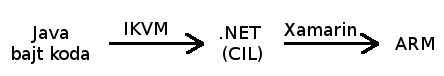
\includegraphics[width=8.5cm]{pic/javabajt.png}
\end{center}
\caption{Grajenje iOS paketa}
\label{libgdxss}
\end{figure} 

\section{PlayN}
\label{sec:playn}
PlayN \cite{playn} je v Javi napisano ogrodje za razvoj grafično intenzivnih aplikacij za različne platforme. Podprte platforme so namizni računalniki (Java), iOS, Android, spletne aplikacije in Flash.

Vmesnik je napisan v programskem jeziku Java. Našo aplikacijo lahko razvijamo na namiznem računalniku, uporabimo pa lahko tudi vroče izmenjavanje kode. 

Za izvoz na različne platforme uporabimo orodje Ant ali Maven. Večjih razlik med orodjema iz perspektive uporabnika ogrodja ni, saj oba omogočata preprost način grajenja domorodnih paketov za Android, iOS, HTML5 in Flash. Za izvoz aplikacije v izvedljivo jar datoteko, ki jo lahko poganjamo na namiznih računalnikih, moramo poskrbeti sami.  

\subsection{Izvoz za iOS naprave}

Za grajenje iOS aplikacije veljajo enake zahteve kot pri LibGDX knjižnici. Java izvorna koda se prevede v CIL, ki se potem s pomočjo Xamarin prevajalnika prevede v ARM izvorno kodo. Ta se potem lahko izvaja na iOS napravah. Orodja Ant ali Maven opravita vse potrebne korake in pripravita projekt, ki ga lahko uvozimo v razvijalsko razvojno okolje Xcode.

\subsection{Izvoz v HTML5 z uporabo GWT}

Izvoz aplikacije v HTML5 je mogoč z uporabo Googlovih spletnih orodij (angl. Google Web Toolkit, GWT). GWT omogočajo razvijanje kompleksnih aplikacij v Javi. Java aplikacija se prevede v JavaScript, ki je optimiziran za posamezne spletne brskalnike. Prevajanje poteka iz izvorne kode v izvorno kodo. Celoten paket vsebuje knjižnico z Java programskim vmesnikom, prevajalnik in strežnik za razvijanje aplikacije.

GWT program napisan v jeziku Java se prevede v optimiziran JavaScript. Prevajalnik upošteva prednosti in slabosti posameznih brskalnikov in optimizira za vsak brskalnik posebej. Poleg brskalnikov za namizje je prevedeni JavaScript optimiziran tudi za mobilne brskalnike, tako da aplikacija napisana s pomočjo GWTja deluje hitreje tudi na mobilnih napravah.

Poleg specifičnih optimizacij za različne brskalnike prevajalnik odstrani tudi mrtvo kodo, optimizira nize znakov in metode pretvori v enovrstično varianto.

\section{Unity}
\label{sec:unity}

Unity3D \cite{unity} je razvojno okolje za izdelovanje medplatformnih grafično intenzivnih aplikacij. Poleg mobilnih naprav (iOS, Android, BlackBerry, Windows Phone 8) ter vseh glavnih namiznih operacijskih sistemov (Windows, MacOS, Linux), orodje omogoča izdelovanje aplikacij tudi za igralne konzole (Xbox in PS3). Orodje je sestavljeno iz dveh glavnih delov - Unity pogon in integrirano razvojno okolje.

\subsection{Pogon}

Za risanje na zaslon Unity uporablja grafični vmesnik Direct3D (na platformi Windows in Xbox) in OpenGL ES (iOS, Android). Pogon omogoča napredne napredne funkcijem, kot so dinamične sence, celozaslonski efekti po procesiranju in renderiranje na teksturo. 

V pogon lahko uvozimo 3D modele v različnih formatih. Podprti so 3ds Max, Blender, Maya in drugi. 

\subsection{Integrirano razvojno okolje} 

Integrirano razvojno okolje razvijalcu omogoči hiter razvoj grafične aplikacije in tudi celovit pregled nad sceno, ki jo trenutno razvija. Razvojno okolje ima dve glavni stanji. Prvo stanje - stanje razvijanja - je namenjeno dodajanju objektov v sceno, spreminjanje njihovih nastavitev, določanje materialov in drugih nastavitev. Drugo stanje - stanje igranja - pa simulira potek izvajanja grafičnega programa in razvijalcu omogoča pregled nad delovanjem aplikacije. 

Izvoz na posamezne platforme poteka preko dialoga za izvoz. V dialogu določimo želeno platformo in nastavitve. Aplikacija se potem prevede in optimizira za izbrano platformo.


\section{Programski jezik Haxe}
\label{sec:haxe}

Programski jezik Haxe \cite{haxe} je bil ustvarjen z razlogom, da bi olajšal razvoj medplatformnih aplikacij. Prevajalnik zna izvorno kodo prevesti na veliko različnih platform. Izvorna koda napisana v jeziku Haxe je lahko prevedena v JavaScript, Adobe Flash, NekoVM, PHP, C++, C\# in Javo.

Jezik Haxe temelji na jeziku C in se zaradi podobnosti drugim jezikom (Java, JavaScript, ActionScript) ni težko učljiv. Haxe je strogo tipiziran, kar pomeni, da prevajalnik že med prevajanjem programa lahko odkrije določene vrste napak. Na voljo je tudi inferenca tipov, generiki in zaprtje funkcij. 

Jezik je odprtokoden in prost za uporabo tako za odprtokodne kot komercialne projekte.

\section{Razvoj medplatformnih aplikacij v programskem jeziku C++}
\label{sec:cpp}
Programski jezik C++ je dostopen povsod. Linux, iOS, OSX in Windows imajo domorodno podporo za C++. Android C++ podpira z orodjem za domoroden razvoj aplikacij (angl. Native Development Kit, NDK), na voljo pa je tudi na platformi iOS. Uporaba jezika C++ za razvoj aplikacij na mobilnih paltformah nam omogoči dostop do sistema za grafiko (OpenGL, oz. Direct3D na Windows), redko pa tudi do elementov za uporabniški vmesnik. Le te na mobilnih napravah praviloma lahko uporabljamo samo iz domorodnih programskih jezikov za določeno platformo ali pa s pomočjo orodij kot je ObjectiveC++, .NET most in Java JNI.

Značilnost grafično intenzivnih aplikacij je v tem, da za svoje delovanje ne potrebujejo veliko elementov za uporabniški vmesnik, saj večinoma tečejo v celozaslonskem načinu. Zato problem iz prejšnjega odstavka ni tako pereč, še posebej, če se zavedamo prednosti, ki jih pridobimo z uporabo C++. 

Prednosti vključujejo eno programsko kodo aplikacije za vse platforme. Le-te ni potrebno prevajati v druge jezike, kot smo videli drugod (razdelki \ref{sec:libgdx}, \ref{sec:haxe}, \ref{sec:playn}) hkrati pa tudi nimamo problemov z učinkovitostjo in slabo podprtostjo (razdelka \ref{sec:2dcanvas}, \ref{sec:WebGL}).

Vseeno se izkaže, da implementacija programskega jezika C++ na posameznih platformah ni povsem enaka. Androidov NDK nima vgrajenih veliko funkcij, ki so drugje standardne. Tak primer so izjeme, ki v NDKju niso podprte in jih moramo dodati sami. Za premostitev razlik med implementacijami se uporabljajo orodja, kot je CMake, ki pred korakom prevajanja poskrbi, da se bodo prevedle tudi vse dodatne knjižnice, ki jih aplikacija potrebuje na določeni platformi.

\subsection{Gameplay}

Projekt Gameplay je odprtokodni 3D grafični pogon, ki deluje na različnih platformah \cite{gameplay}. Pogon razvija podjetje Blackberry, ki s projektom želi vzpodbuditi razvoj za njihove naprave. Poleg BlackBerry naprav so podprte še iOS od verzije 5 naprej, Android od verzije 2.3 dalje, Windows 7, OSX in Linux. Mobilne naprave z operacijskim sistemom Windows niso podprte.

Poleg metod za dostop do OpenGL ES 2.0 knjižnice na mobilnih napravah, oziroma OpenGL 3.2 na namiznih računalnikih, ima projekt vgrajen tudi generator terenov, graf scene, sistem za računanje fizike, deklarativen sistem za uporabniški vmesnik, podprt pa je tudi skriptni jezik Lua.

Grajenje medplatformnih aplikacij omogoča orodje CMake, ki poskrbi za vse pritikline na posameznih platformah. 

\subsection{OGRE}
\label{sec:ogre}
OGRE (Object-Oriented Graphics Rendering Engine) \cite{ogre} je pogon za upodabljanje napisan v programskem jeziku C++. Prednost pogona je, da nam ponudi enoten vmesnik tako za OpenGL kot Direct3D. OGRE podpira večino različnih sistemov Linux, Windows (tudi Phone in RT), OSX, iOS in Android.

Prednost OGRE pred drugimi podobnimi projekti je tudi, da ima zelo dobro dokumentacijo in da se striktno drži standardov programiranja. Tudi na splošno je pogon dobro zamišljen in konsistenten.

OGRE ima preprost objektno orientiran vmesnik, ki poenostavi delo ustvarjanja 3D scen.

\subsection{Marmalade}
\label{sec:marmalade}
Marmelade \cite{marmalade} je zanimivo orodje, ki nam omogoča pisanje medplatformnih aplikacij v jeziku C++, JavaScript ali pa s programskim jezikom Lua. Izbira jezika je odvisna od naših preferenc in zahtevnosti projekta.

Orodje Marmalade ni na voljo brezplačno, brez plačila je na voljo samo 30 dnevna verzija. Cena najbolj osnovne licence, ki nam omogoča grajenje aplikacij za platforme iOS in Android je \$15 na mesec. Če pa bi želeli podpreti še BlackBerry in Windows Phone pa cena naraste na \$499 na leto.

Marmalade nudi direkten dostop do OpenGL ES vmesnika API, pester nabor možnosti za razvoj uporabniških vmesnikov in kompatibilnost z popularnimi knjižnicami za C++. 

Orodje Marmalade je sestavljeno iz dveh delov. Prvi je Marmalade sistem, ki je plast abstrakcije za delo z operacijskim sistemom. Drugi pa Marmalade studio, ki je komplet orodij za delo z 2D in 3D grafiko. Moduli skrbijo za 2D in 3D izris, renderiranje modelov in bitmap pisave.

Za grajenje medplatformnih aplikacij se uporabljajo MKB datoteke, v katere se za vsako platformo zapišejo nastavitve, kot so na primer katere datoteke naj se vključijo, definicije za predprocesor in nastavitve za izvoz na naprave. Iz izvorne kode aplikacije se ustvari platformno neodvisna binarna datoteka. To binarno datoteko potem s priloženim orodjem za izvoz lahko izvozimo na želene platforme.

\section{Monogame}

Monogame je orodje, ki lahko obstoječe aplikacije pisane za platforme Windows in Windows Phone, pripravi še za druge platforme. Trenutno podprti sistemi so OSX, Linux, iOS, Android, Play Station Mobile in Ouya. 

Sprva je Monogame podpiral samo prevedbo 2D aplikacij, vendar je dobil podporo za 3D programski vmesnik z verzijo 3.0.0. Cilj projekta je v celoti podpreti XNA 4 vmesnik API. Za prevod obstoječe aplikacije na iOS in Android se uporablja Xamarin platforma (razdelek \ref{sec:xamarin}), kar pomeni, da moramo pridobiti dve licenci. Verzija 3.0.0 je osredotočena na funkcije, ki jih prinaša OpenGL ES 2.0, medtem ko so prejšnje verzije temeljile na OpenGL ES 1.X. Na Windows sistemih se namesto OpenGLa uporablja Direct3D.

\section{Adobe Flash}

Adobe Flash \cite{flash}, znan tudi pod imeni Shockwave Flash in Macromedia Flash, je uporabnikom najbolj poznan v obliki vtičnika za spletne brskalnike. Začetki segajo v leto 1995, ko je bil razvit kot vtičnik za animacije na spletnih straneh. Matično podjetje je nato kupila Macromedia, ki pa se je kasneje prodala Adobeju.   

Od Flash verzije 11 naprej ima predvajalnik podporo tudi za strojno pospeševanje 3D vsebin.

Podpora na mobilnih platformah je slaba, saj iOS Flasha nikoli ni podpiral, na Androidu pa je od verzije 4.0 uradno ni več podprt, neuradno je možno Flash predvajalnik namestiti tudi na Android sistemih 4.1 in 4.2. Zaradi slabih smernic Flash ni najbolj primeren za razvoj grafično intenzivnih aplikacij.

Probleme s slabo podporo lahko nekoliko premostimo z uporabo vmesnikov, ki aplikacijo znajo zapakirati, kot domorodne aplikacije za posamezne platforme.

\subsection{Stage3D in Starling}

Programski vmesnik Stage3D nam mogoča strojno pospešeno arhitekturo, ki deluje na več platformah. 

Starling je odprto koden projekt, ki temelji na Stage3Dju. Nad stage3D doda dodatno funkcionalnost kot so sistem za dogodke, podpora partiklom, podpora različnim teksturam, teksturni atlasi, različni načini blendanja in podpora za več večprstne dotike.

\section{QT}
\label{sec:qt}
% http://doc-snapshot.qt-project.org/qt5-stable/qtdoc/windowsce-opengl.html

Projekt QT je medplatformno ogrodje za ustvarjanje aplikacij. Za razvijanje aplikacij sta na voljo C++ in QML, ki je jezik podoben JavaScriptu in CSSu.

Za razvijanje aplikacij je na voljo tudi vgrajeno razvijalno okolje QT Creator.

Qt je možno uporabljati na velikem številu različnih naprav naprav in platform z uporabo različnih CPU arhitektur. QT skupnost med drugimi podpira tudi naprave Beagleboard (razdelek \ref{sec:beagleBone}) in RaspberryPi (razdelek \ref{sec:raspberryPi}). 

iOS in Android sta trenutno podprta samo eksperimentalno in ni še jasno, kdaj bo podpora postala stabilna.% Razvija se pa tudi vprašanje o domorodnih QT Android sistemih. % http://qt-project.org/wiki/native-Android-discussion